\chapter{材料力学的一些基本}
\intro{
	在看清了世界的荒诞与冷峻之后，依然选择报之以歌。
	
	\rightline{——Albert Camus}
}
\section{基本任务}
在实际工程中，构件应满足如下需求：
\begin{enumerate}
	\item 强度要求：在规定载荷作用下的构件不应破坏。
	\item 刚度要求：有足够的抵抗变形的能力。
	\item 稳定性要求：有足够的保持原有平衡形态的能力。
\end{enumerate}

于是，我们需要研究一维杆件的承载能力。

\section{基本假设}
为了研究方便，我们引入一些基本假设来简化模型：
\begin{enumerate}
	\item[连续性假设] 认为组成固体的物质不留间隙地充满了固体的体积。这是对坐标增量进行极限分析的基础。\\
	\item[均匀性假设] 认为固体内处处有相同的力学性能。\\
	\item[各向同性假设] 认为固体的力学性能与方向无关。\\
	\item[小变形假设] 认为变形的尺寸远小于原尺寸。
\end{enumerate}


\section{基本变形形式}
\begin{enumerate}
	\item 轴向拉伸或轴向压缩
	\item 剪切
	\item 扭转
	\item 弯曲
\end{enumerate}
\section{基本研究对象}
杆，轴，柱，梁

\section{基本概念}
\subsection{内力}
\begin{definition}
	变形引起的内部附加力。
\end{definition}
 	内力是由变形引起的，没有变形没有内力。
 	在理论力学里，因为刚体假设，物体内部不产生变形，所以不考虑内力。
 	
 	但材料力学研究物体的变形形式，内力的分析就十分重要。
 	
 	内力的分析方法：
 	
 	{\huge{截\ 取\ 代\ 平}}
 \subsection{应力}
 若将内力向一点进行简化，由理论力学，我们有平面力系的简化定理，这是可以做到的。
 
 但是，简化后的力矢和力矩只能反应平衡关系，不能体现内力在截面内某一点的强弱程度。于是我们引入内力集度的概念。
 就是我们所说的应力。
 
 \begin{definition}
 	$p = \lim_{\Delta A \to 0} \frac{\Delta F}{\Delta A}$
 \end{definition}
 
 \begin{figure}[htbp]
 	\centering
 	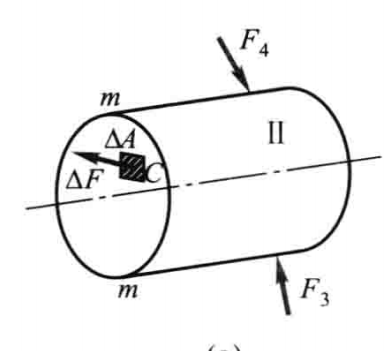
\includegraphics[width=0.15\linewidth]{Figure/应力.png}
 \end{figure}
 
 \subsection{应变}
 \begin{figure}[htbp]
 	\centering
 	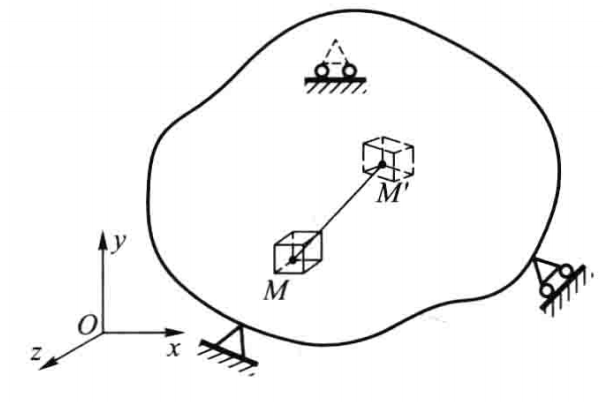
\includegraphics[width=0.5\linewidth]{Figure/线应变.png}
	\caption{线应变示意图}
 \end{figure}
 \begin{definition}
	$\varepsilon =\lim_{x \to 0} \frac{\Delta s}{\Delta x}$  
 \end{definition}

 其中，$\varepsilon$ 称为沿 $x $ 方向的线应变或正应变。
